%**************************************************************************************
% License:
% CC BY-NC-SA 4.0 (http://creativecommons.org/licenses/by-nc-sa/4.0/)
%**************************************************************************************

\documentclass[notes]{beamer}

\mode<presentation> {

\usetheme{Madrid}

% Burnt orange
\definecolor{burntorange}{rgb}{0.8, 0.33, 0.0}
\colorlet{beamer@blendedblue}{burntorange}
% Pale yellow
\definecolor{paleyellow}{rgb}{1.0, 1.0, 0.953}
\setbeamercolor{background canvas}{bg=paleyellow}
% Secondary and tertiary palett
\setbeamercolor*{palette secondary}{use=structure,fg=white,bg=burntorange!80!black}
\setbeamercolor*{palette tertiary}{use=structure,fg=white,bg=burntorange!60!black}

% To remove the footer line in all slides uncomment this line
%\setbeamertemplate{footline}
% To replace the footer line in all slides with a simple slide count uncomment this line
%\setbeamertemplate{footline}[page number]

% To remove the navigation symbols from the bottom of all slides uncomment this line
%\setbeamertemplate{navigation symbols}{}
}

\usepackage{amsmath}
\usepackage{bm}
\usepackage{breqn}
\usepackage{graphicx} % for figures
\usepackage{subcaption} % for subplots 
\usepackage[labelsep=space,tableposition=top]{caption}
\renewcommand{\figurename}{Fig.} 
\usepackage{cleveref}
\usepackage{caption,subcaption}% http://ctan.org/pkg/{caption,subcaption}
\usepackage{booktabs} % Allows the use of \toprule, \midrule and \bottomrule in tables


% To print 2 slides on a page
%\usepackage{handoutWithNotes}
%\pgfpagesuselayout{2 on 1}[border shrink=2mm]
%----------------------------------------------------------------------------------------
%	TITLE PAGE
%----------------------------------------------------------------------------------------
% The short title appears at the bottom of every slide, the full title is only on the title page
\title[CE394M: isoparametric - gauss integration]{CE394M: Isoparametric elements and Gauss integration} 
\author{Krishna Kumar} % name
\institute[UT Austin] % institution 
{
University of Texas at Austin \\
\medskip
\textit{
  \url{krishnak@utexas.edu}} % Your email address
}
\date{\today} % Date, can be changed to a custom date

\begin{document}

\begin{frame}
\titlepage % title page as the first slide
\end{frame}

\begin{frame}
 % Table of contents slide, comment this block out to remove it
 \frametitle{Overview}
 % Throughout your presentation, if you choose to use \section{} and \subsection{} 
 % commands, these %will automatically be printed on this slide as an overview 
 \tableofcontents
\end{frame}

%----------------------------------------------------------------------------------------
% slides
%----------------------------------------------------------------------------------------
\section{Rectangular elements}
%------------------------------------------------
\begin{frame}
\frametitle{4-noded rectangulr element}
\begin{figure}[ht]
	\centering
	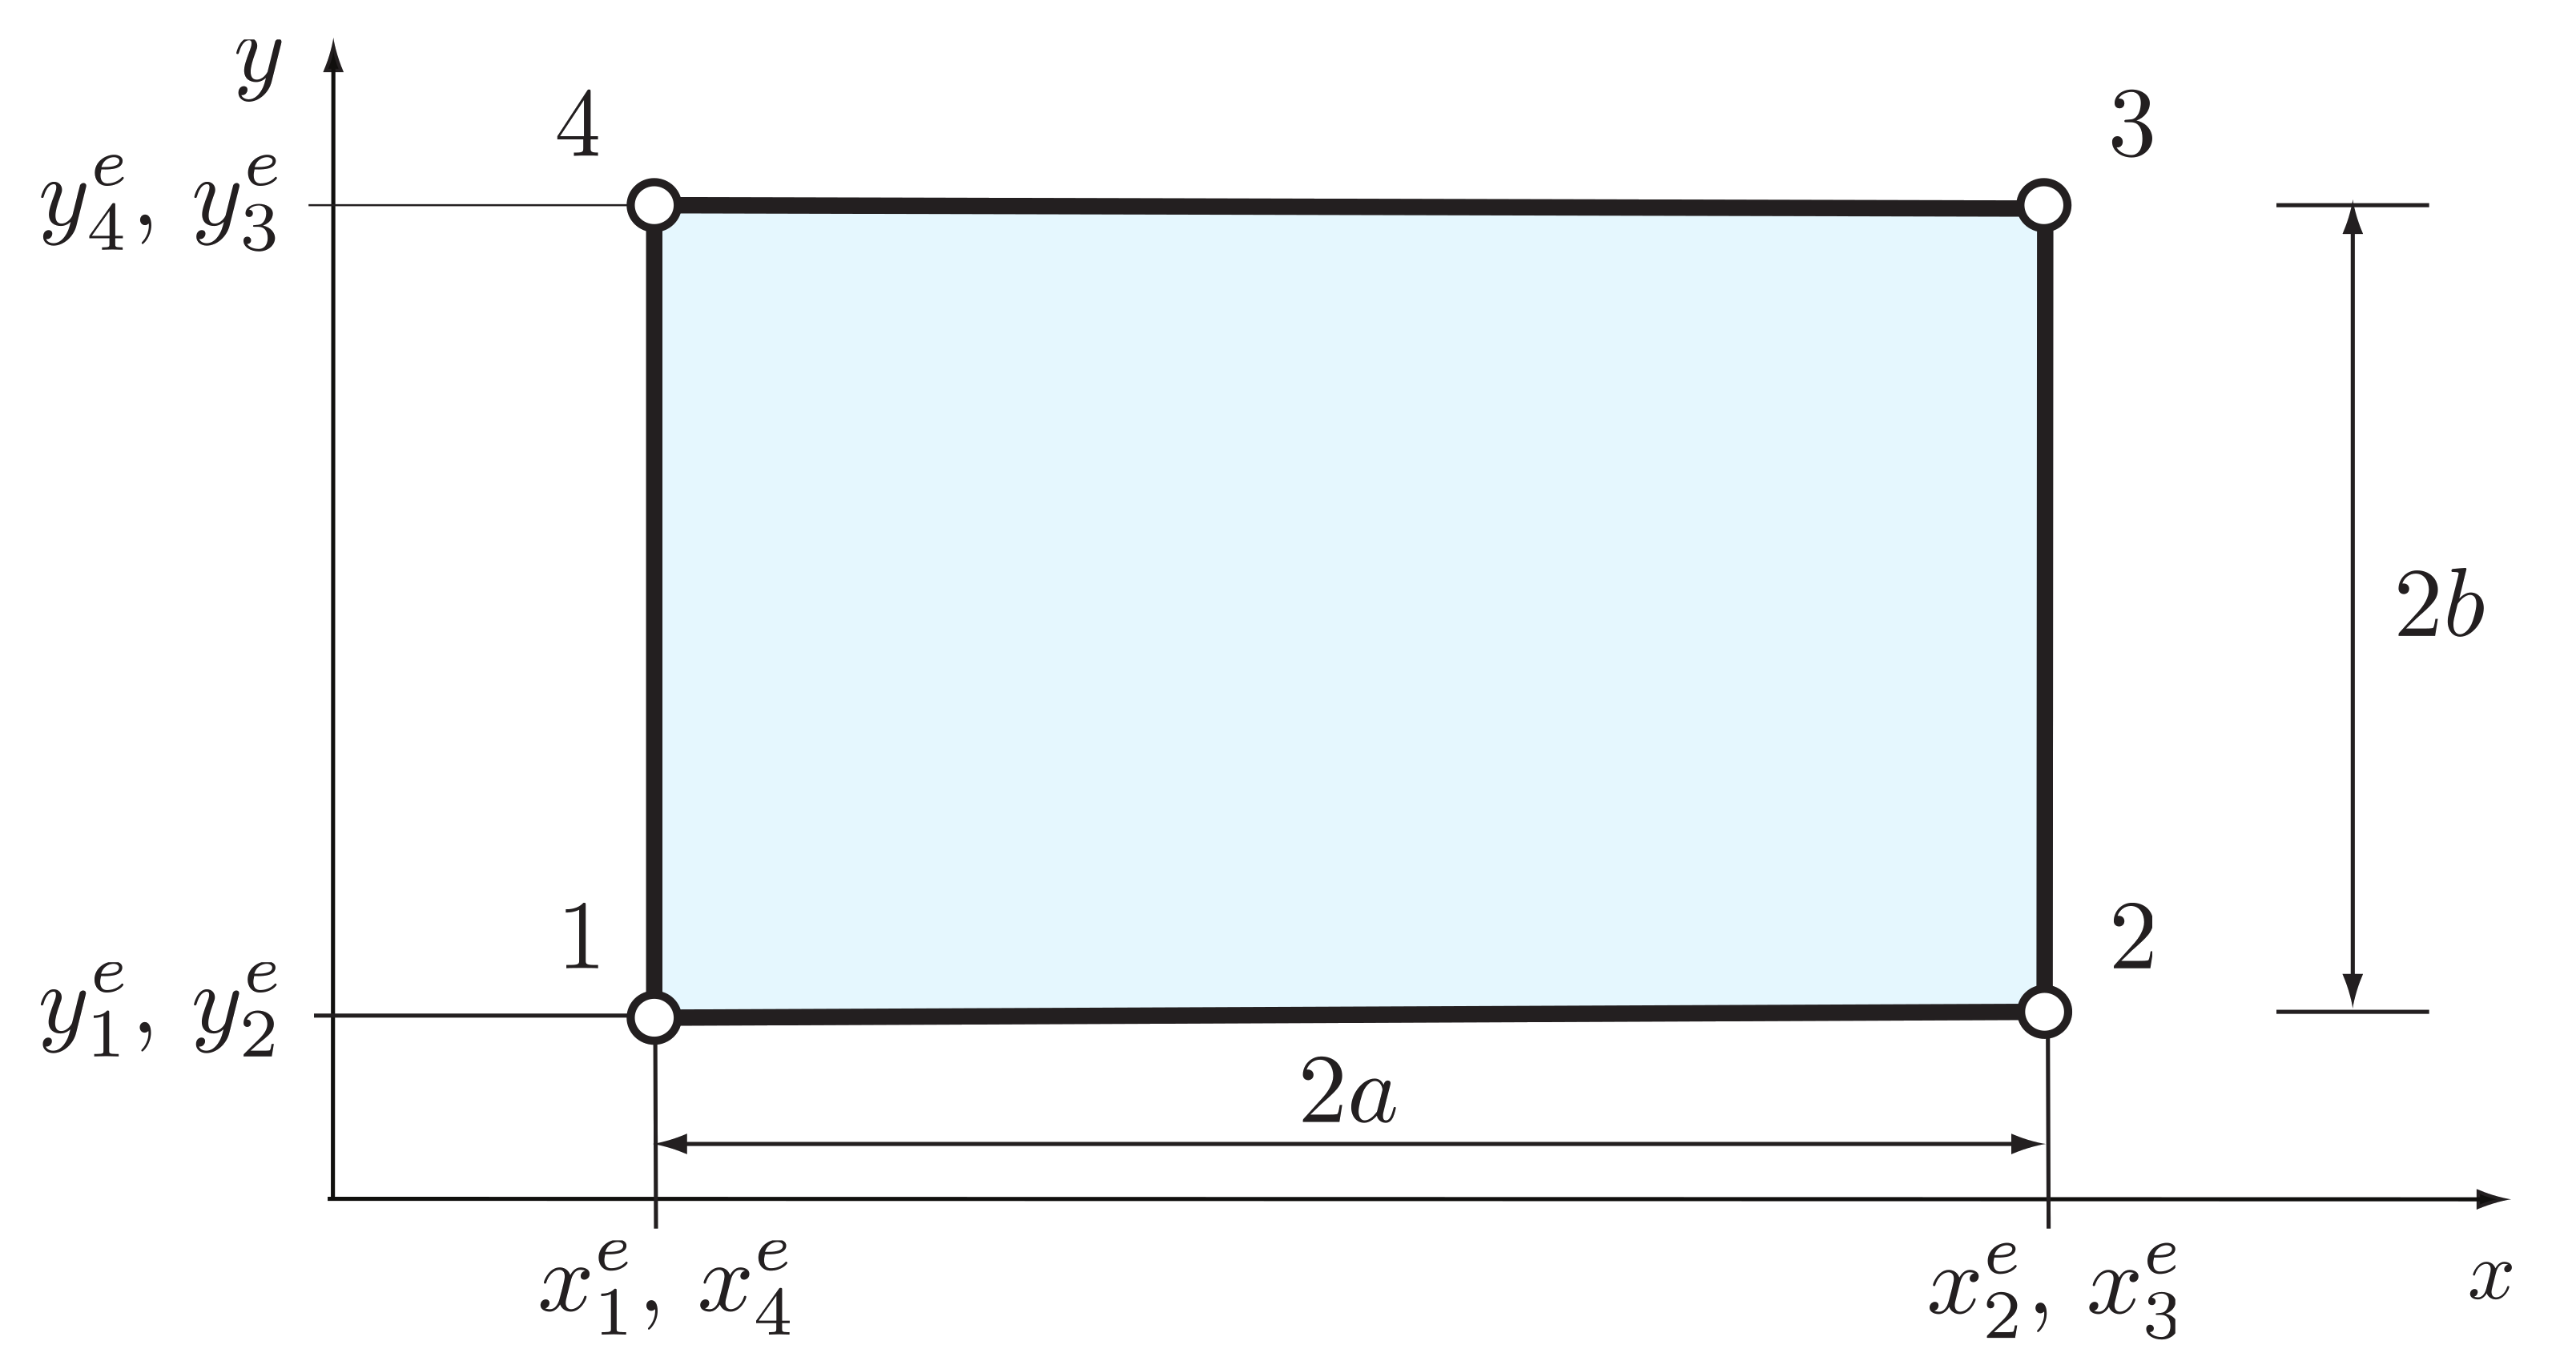
\includegraphics[width=0.85\textwidth]{figs/four-noded-quadrilateral.png}
	\caption*{Four-node rectangular element. The nodes are by definition numbered counter-clockwise.}
\end{figure}
\end{frame}

%------------------------------------------------
\begin{frame}
\frametitle{4-noded rectangular element}
As the element has four nodes, it is necessary to start with a polynomial that has four
parameters.
\mode<beamer>{
	\begin{equation*}
			T e = \alpha_0^e + \alpha_1^e x + \alpha_2^e y + \alpha_3^e xy
	\end{equation*}
	It is possible to express ($\alpha_0^e, \alpha_1^e, \alpha_2^e, \alpha_3^e$) in terms of the nodal values ($T_1^e, T_2^e, T_3^e , T_4^e$). A derivation shape functions is tedious as it is necessary to invert a 4 x 4 matrix.
	
	The Shape Functions should be 1 at each node, and 0 otherwise can be used to determine the 4 coefficients.
}
\mode<handout>{
	\vspace{5cm}
}
\end{frame}


%------------------------------------------------
\begin{frame}
\frametitle{4-noded rectangular element}
An alternative and more elegant approach is to construct the shape functions by the \textbf{tensor
product method.} This is based on taking products of one-dimensional shape functions.

\begin{figure}[ht]
	\centering
	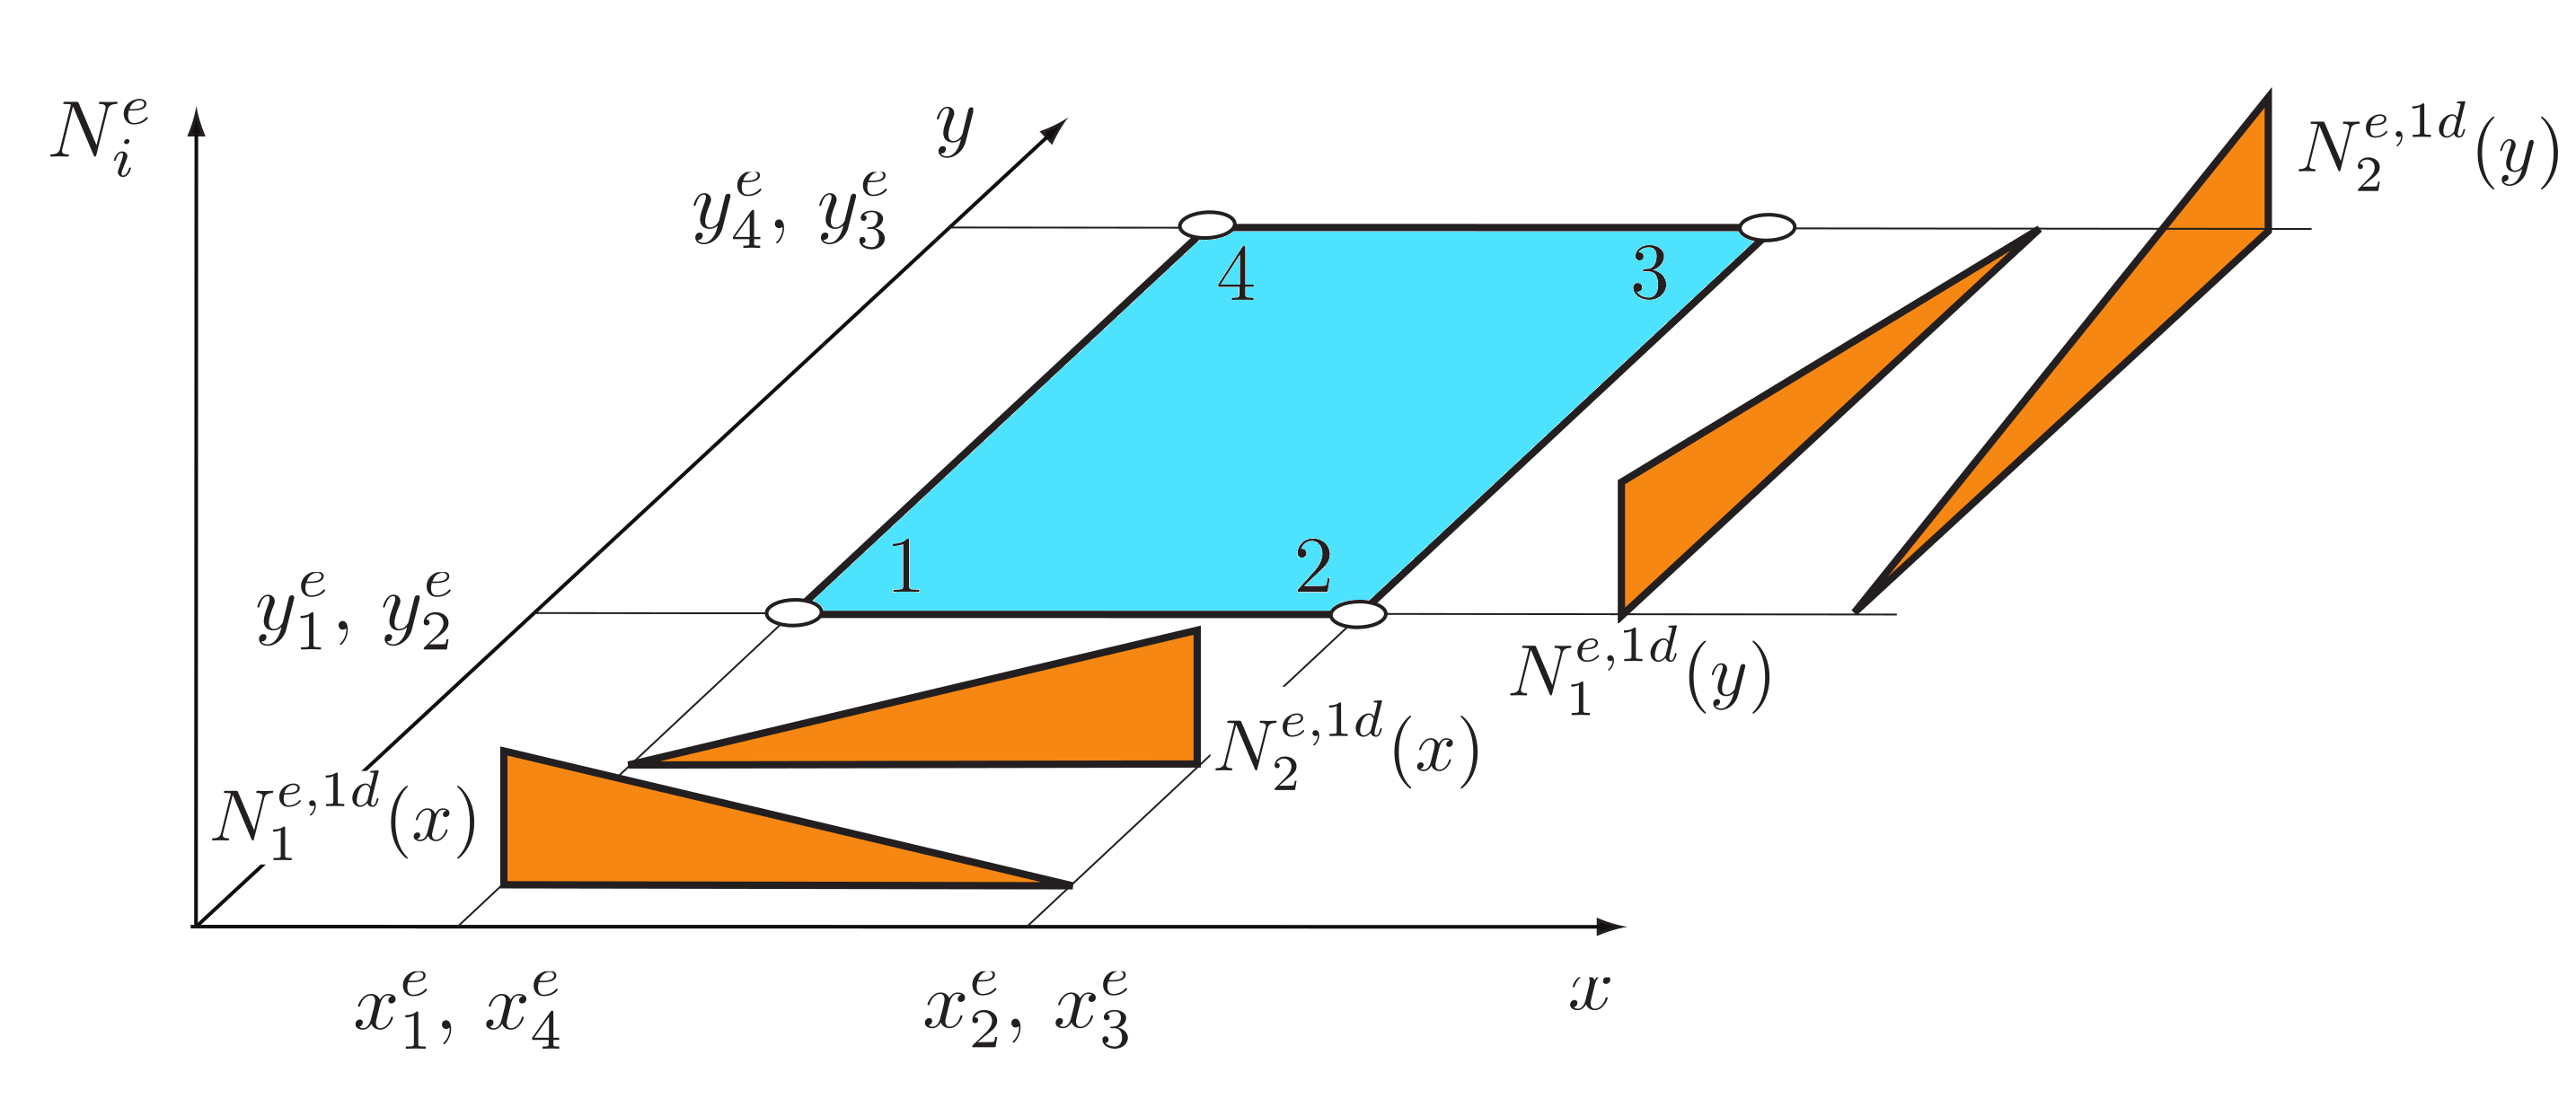
\includegraphics[width=\textwidth]{figs/4noded-quad-tensor-product.png}
	\caption*{Construction of two dimensional shape functions.}
\end{figure}

\end{frame}


%------------------------------------------------
\begin{frame}
\frametitle{4-noded rectangular element}
For example, $N_2^e$, which has to have the value one at node 2 and zero at the other nodes,
is obtained by taking the product of the one-dimensional shape functions $N_2^{e,1d}(x)$ and 
$N_1^{e,1d}(y)$.

\mode<beamer>{
	\begin{equation*}
	N_2^e = N_2^{e,1d}(x) \times N_1^{e,1d}(y)
	\end{equation*}
	
	As visible in the figure above the product $ N_2^{e,1d}(x) \times N_1^{e,1d}(y)$ has the 
	value one at node 2 and is zero at nodes 1, 3 and 4.
	
	\begin{equation*}
	N_2^e (x, y) = \frac{x - x_1^e}{x_2^e - x_1^e}\frac{y - y_4^e}{y_1^e - y_4^e} = -\frac{1}{A^e}(x - x_1^e)(y - y_4^e)
	\end{equation*}
}
\mode<handout>{
	\vspace{5cm}
}
\end{frame}


%------------------------------------------------
\begin{frame}
\frametitle{4-noded rectangular element}

The four shape functions, also called \textbf{bilinear shape functions}, for the quadrilateral element are:
\begin{align*}
	N_1^e (x, y) & = \frac{x - x_2^e}{x_1^e - x_2^e}\frac{y - y_4^e}{y_1^e - y_4^e} = -\frac{1}{A^e}(x - x_2^e)(y - y_4^e) \\
	%
	N_2^e (x, y) & = \frac{x - x_1^e}{x_2^e - x_1^e}\frac{y - y_4^e}{y_1^e - y_4^e} = -\frac{1}{A^e}(x - x_1^e)(y - y_4^e) \\
	%
	N_3^e (x, y) & = \frac{x - x_1^e}{x_2^e - x_1^e}\frac{y - y_1^e}{y_4^e - y_1^e} = -\frac{1}{A^e}(x - x_1^e)(y - y_1^e) \\
	%
	N_4^e (x, y) & = \frac{x - x_2^e}{x_1^e - x_2^e}\frac{y - y_1^e}{y_4^e - y_1^e} = -\frac{1}{A^e}(x - x_2^e)(y - y_1^e)\\
\end{align*}

where $A^e$ is the area of the element.

\end{frame}


%------------------------------------------------
\begin{frame}
\frametitle{4-noded rectangular element}
The four shape functions are plotted in the following
figure:
\begin{figure}[ht]
	\centering
	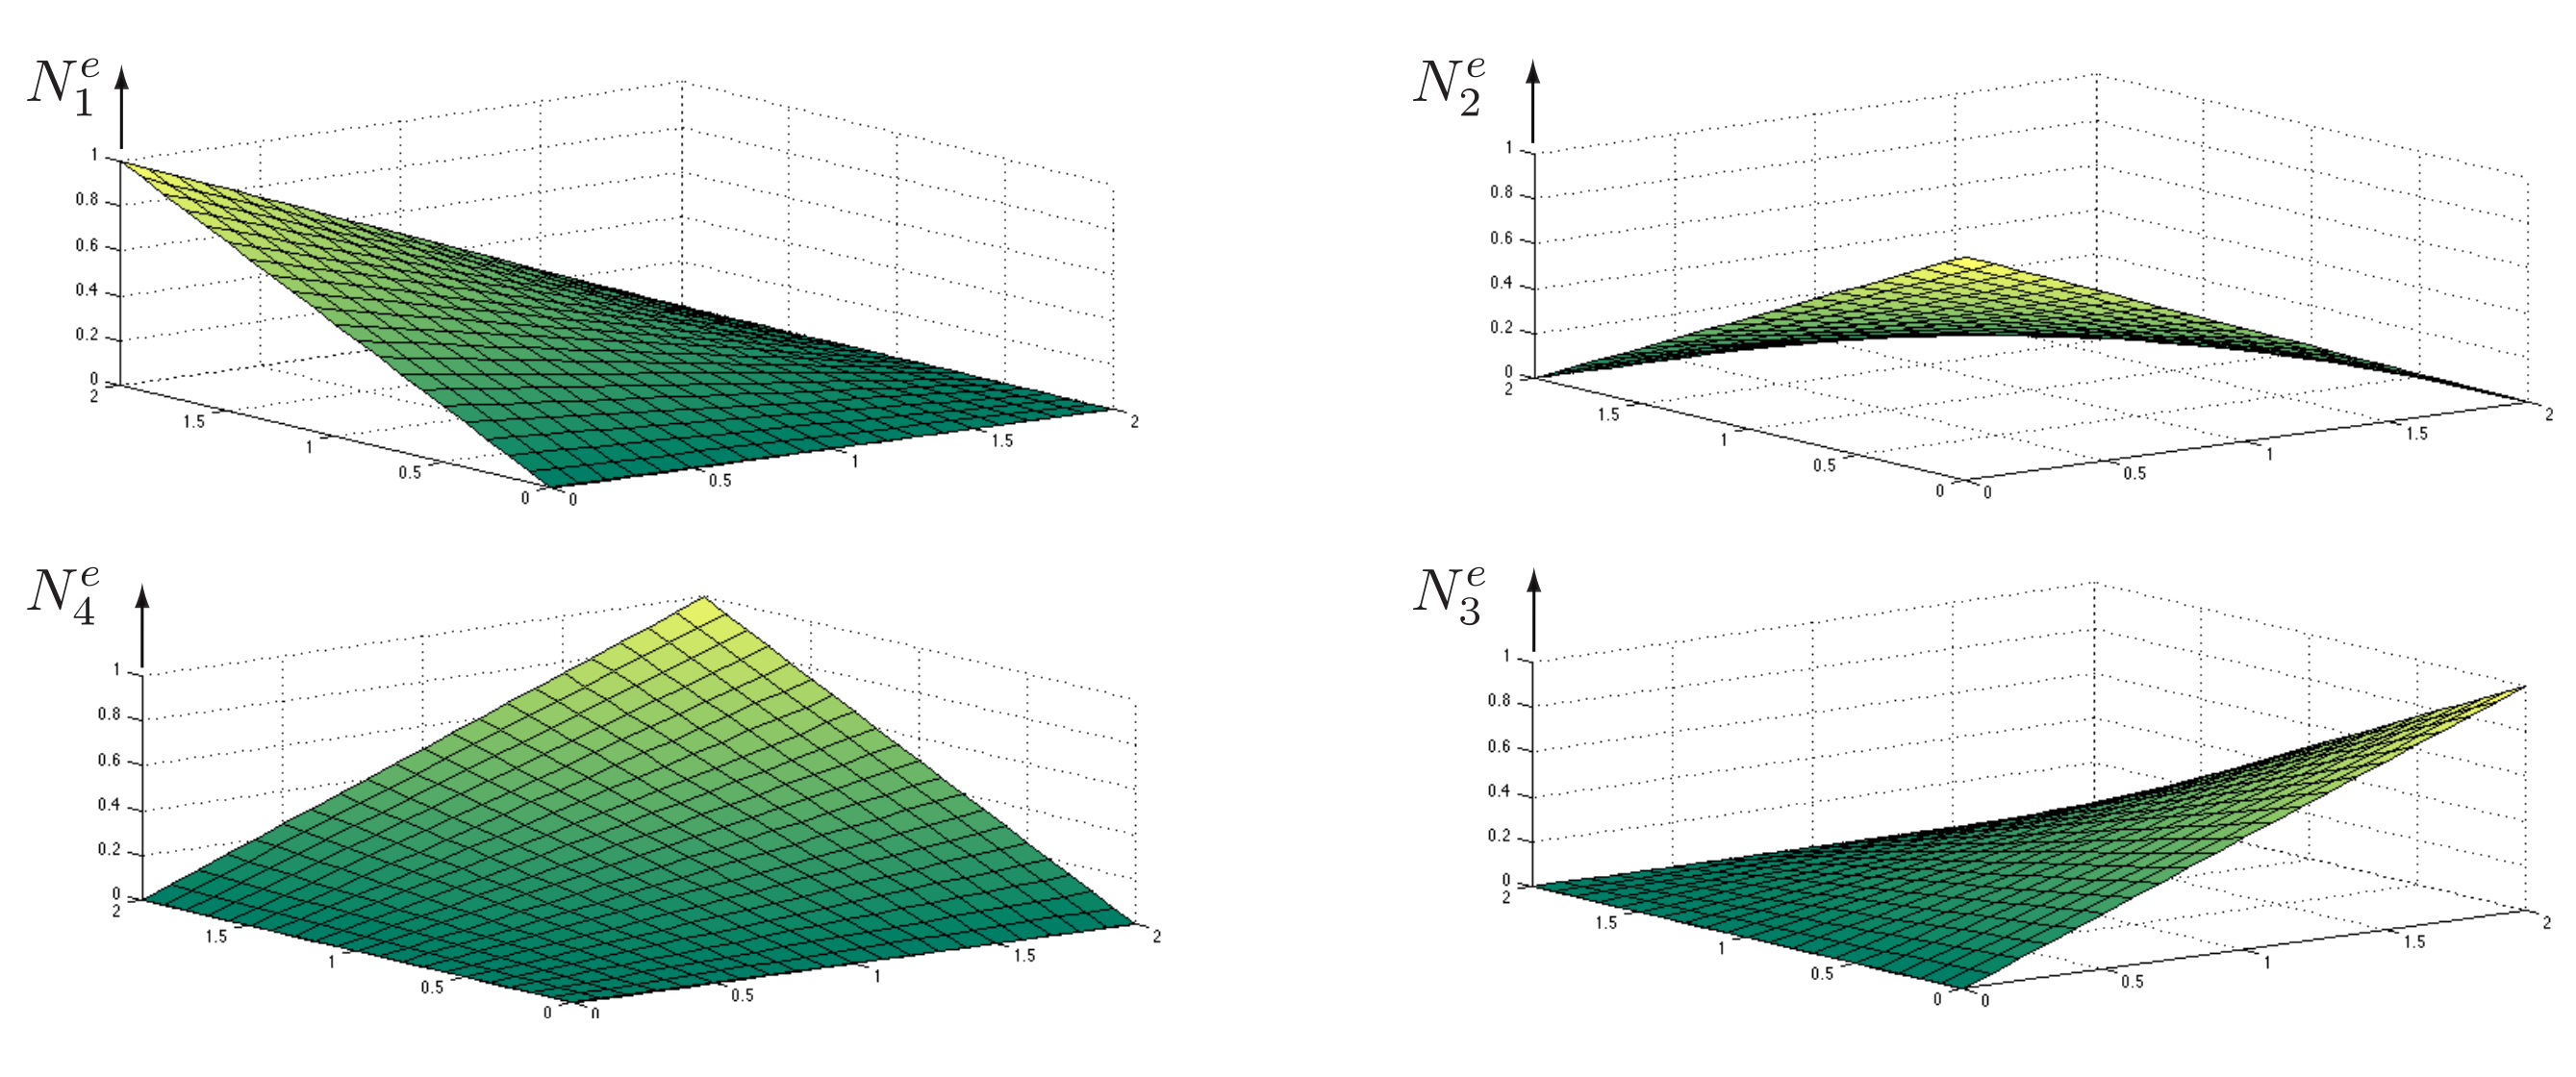
\includegraphics[width=\textwidth]{figs/4noded-sf.png}
	\caption*{Four shape functions of the rectangular element (on $[0, 2] \times [0, 2]$).}
\end{figure}
\end{frame}


%------------------------------------------------
\begin{frame}
\frametitle{4-noded rectangular element}
If the sf equations are used for interpolating the temperature field over arbitrary quadrilaterals, the scalar field (e.g., temperature) across the element boundaries will be not continuous.
\begin{figure}[ht]
	\centering
	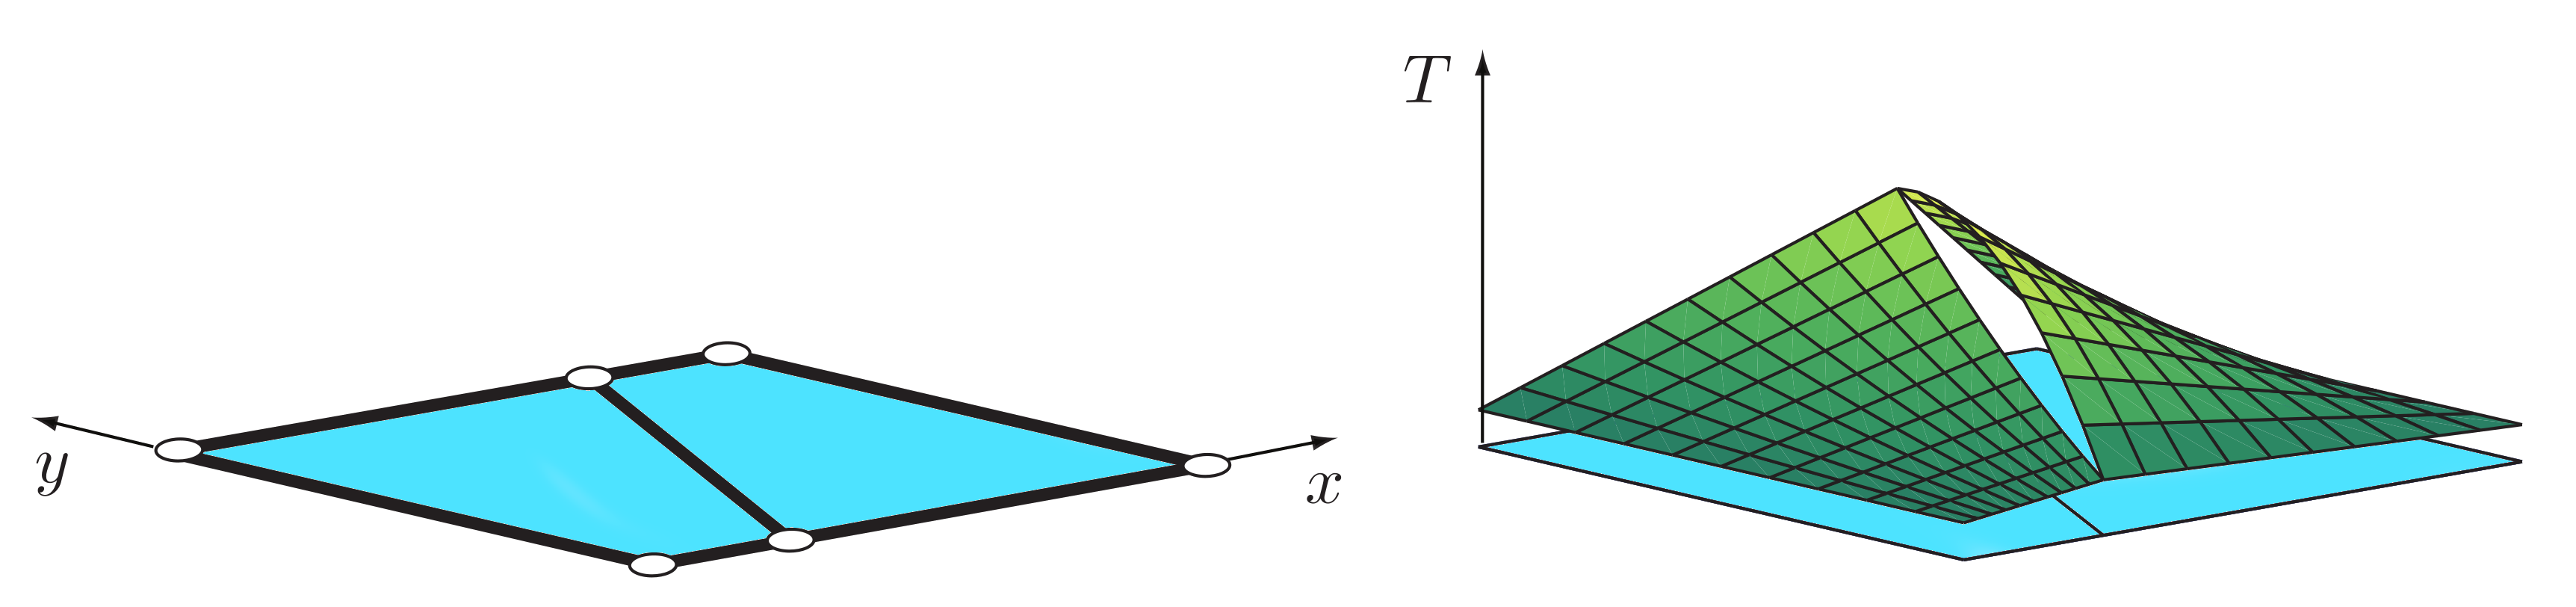
\includegraphics[width=\textwidth]{figs/discontinous-rectangle.png}
	\caption*{Two element mesh with rectangle shape functions. Although the two nodal values on the
		edge agree, the temperature distribution is still discontinuous.}
\end{figure}
\end{frame}

\note{
	The computed shape functions are suitable for rectangles and could be used with meshes consisting only of rectangles, but they are not suitable for arbitrary quadrilaterals.
	
	Therefore, these shape functions are of limited use for practical applications. To obtain
	the shape functions for arbitrary quadrilaterals we need to visit the idea of isoparametric
	mapping.
}

%------------------------------------------------
\section{Isoparametric elements}
%------------------------------------------------
\begin{frame}
\frametitle{Isoparametric mapping in 1D}
\mode<beamer>{
	\begin{figure}[ht]
		\centering
		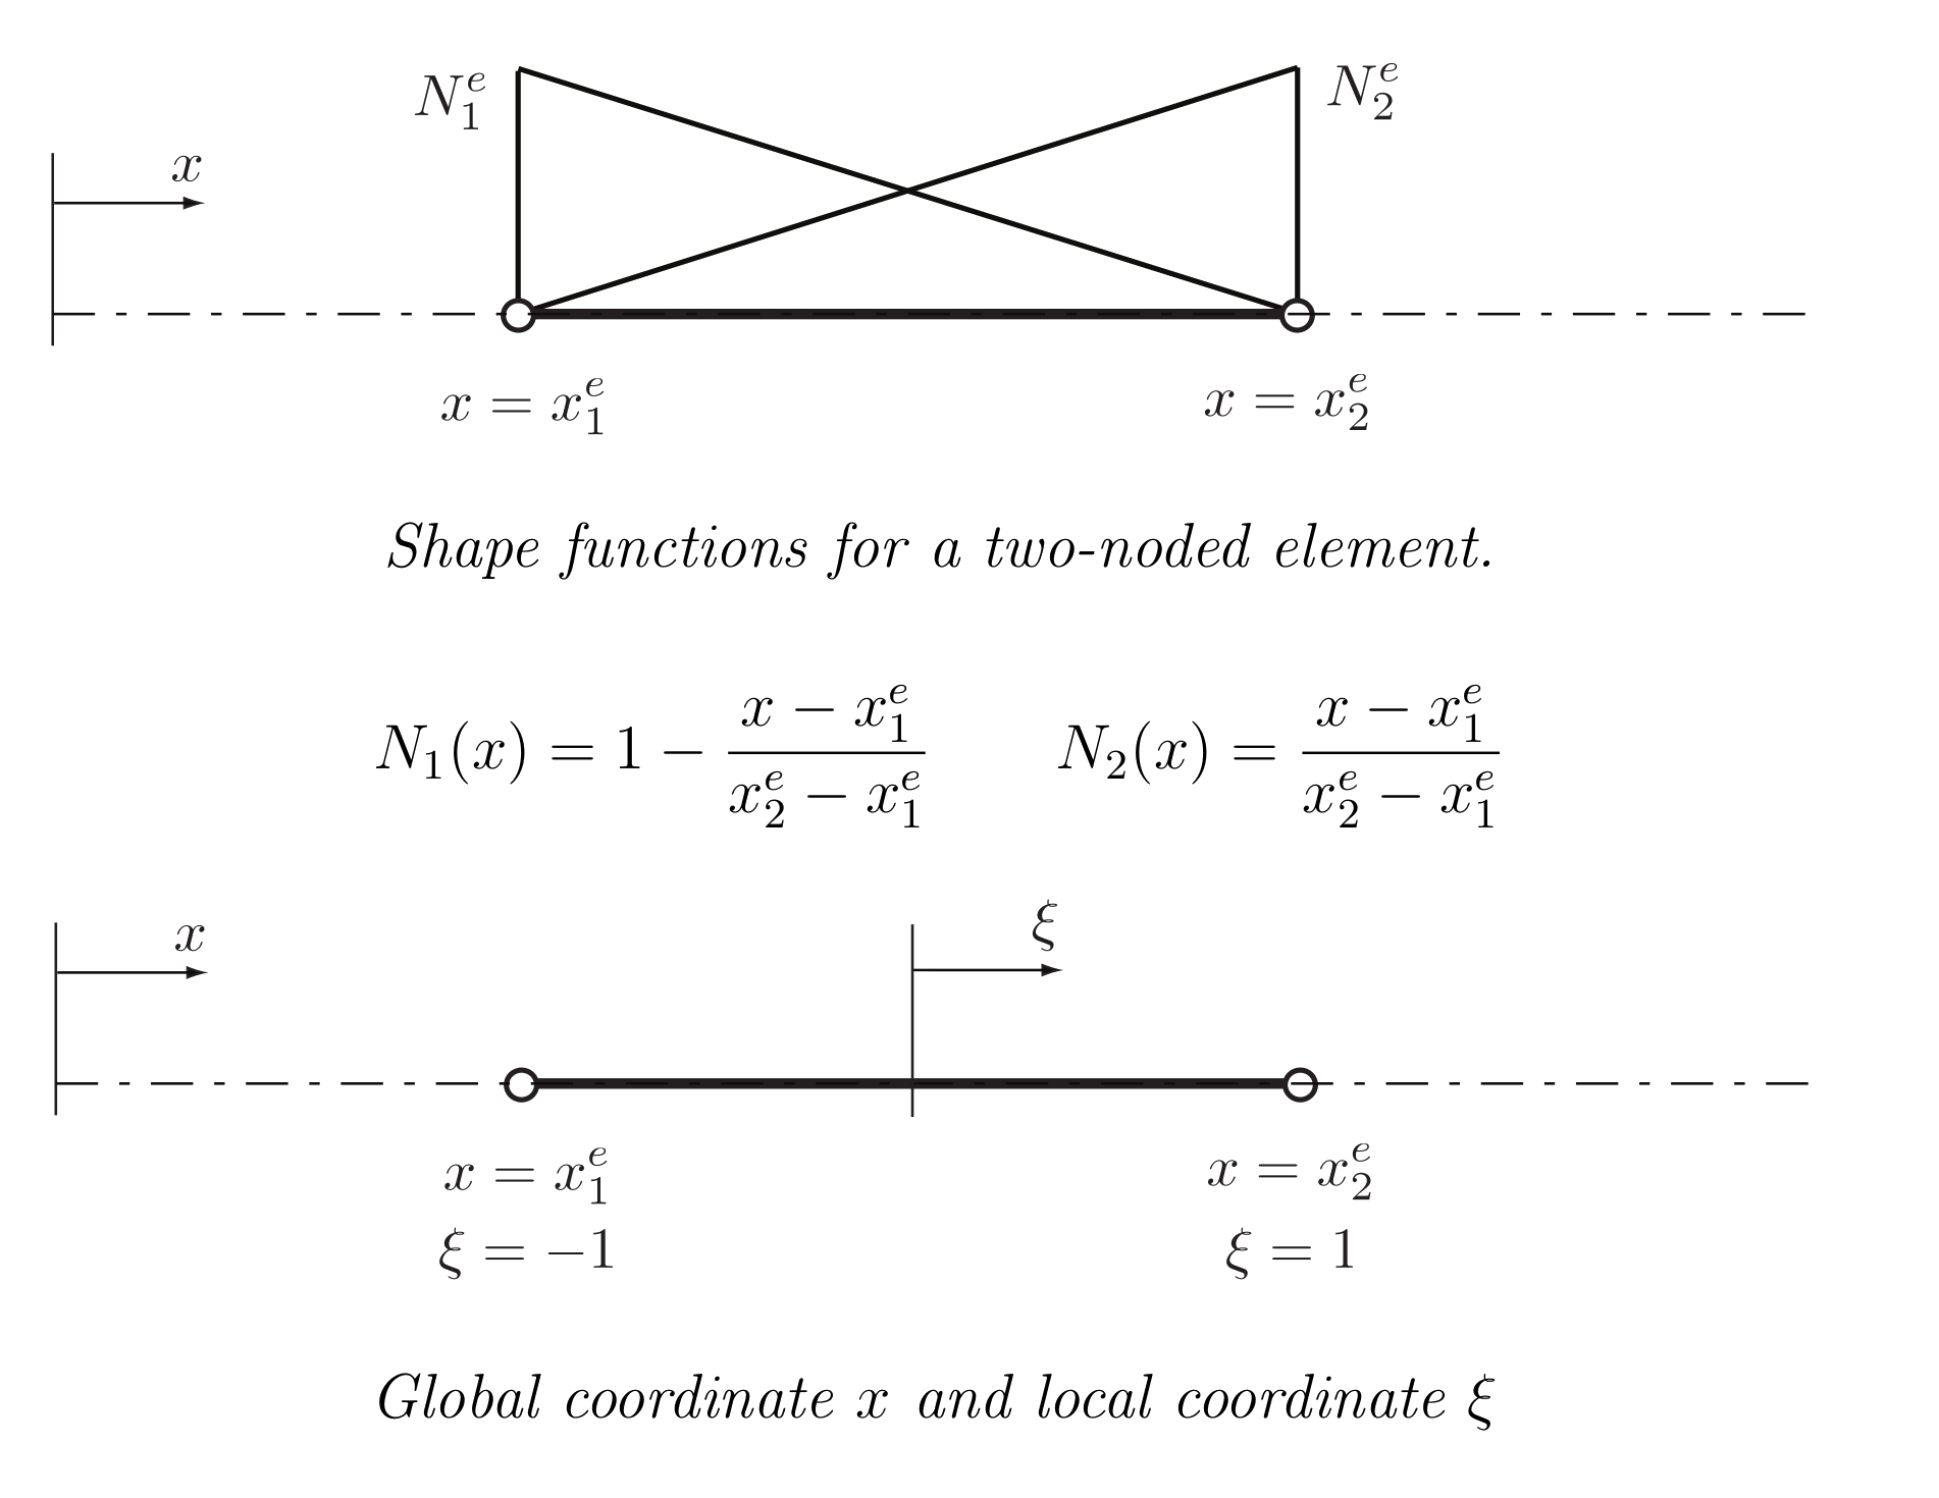
\includegraphics[width=0.85\textwidth]{figs/1d-isoparametric.png}
	\end{figure}
}
\mode<handout>{
	\vspace{5cm}
}
\end{frame}

%------------------------------------------------
\begin{frame}
\frametitle{Isoparametric mapping in 1D}
\mode<beamer>{
	\begin{figure}[ht]
		\centering
		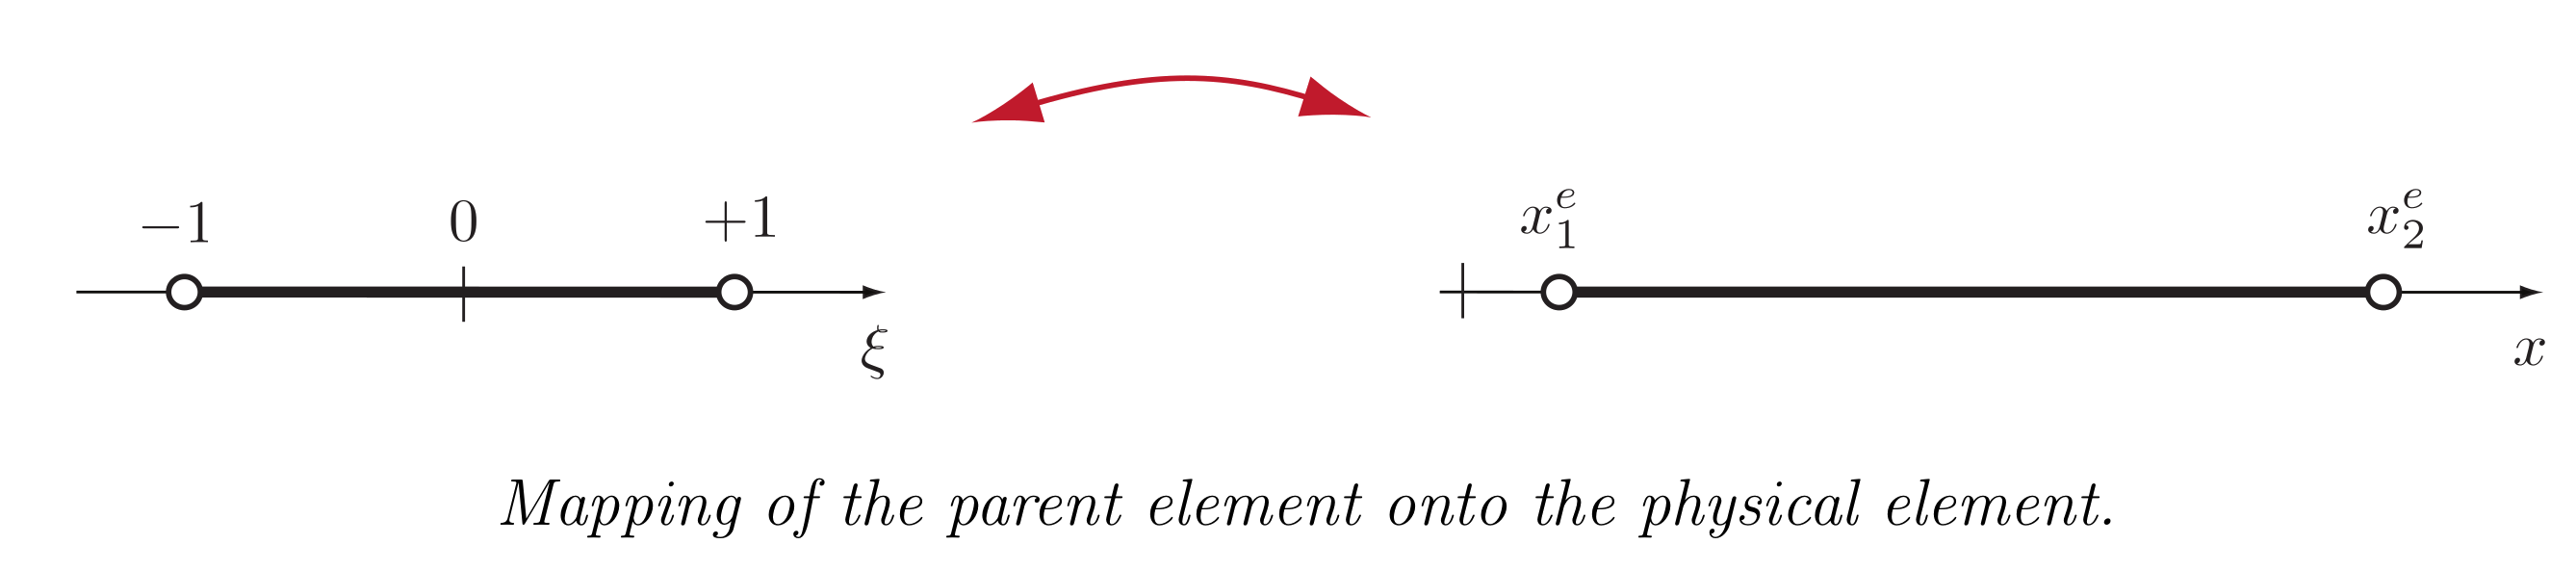
\includegraphics[width=0.85\textwidth]{figs/1d-isoparametric-shapefn.png}
	\end{figure}
}
\mode<handout>{
	\vspace{5cm}
}
\end{frame}
\end{document} 


